\documentclass{standalone}
\usepackage{circuitikz}
\usepackage{schemabloc}

\begin{document}
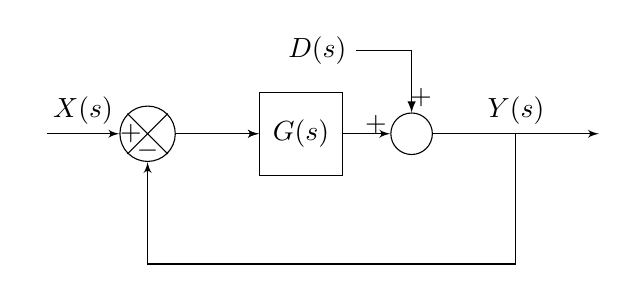
\begin{tikzpicture}
% Entrée principale
\sbEntree{E}
\sbComp{comp}{E}
\sbRelier[$X(s)$]{E}{comp}

% Bloc de transfert principal
\sbBloc[3]{B1}{$G(s)$}{comp}
\sbRelier{comp}{B1}

% Sortie principale


% Perturbation ajoutée en sortie
\sbCompSum*{comp2}{B1}{+}{}{+}{}



\sbSortie[6]{S}{comp2}
\sbRelier[$Y(s)$]{comp2}{S}

\draw[latex-] (comp2)|- ++
(-2em,3em)node[left]{$D(s)$};

% Rétroaction vers le comparateur
\sbRelier{comp}{B1}
\sbRelier{B1}{comp2}
\sbRenvoi{comp2-S}{comp}{}
\end{tikzpicture}
\end{document}
